% Chapter 1

\chapter{Introduction} % Chapter title

\label{ch:introduction} % For referencing the chapter elsewhere, use \autoref{ch:introduction} 

While combinatorics and commutative algebra have both long existed as independent mathematical disciplines, their applications to each other have only become apparent in recent decades. Richard Stanley, considered to be the father of the field of combinatorial commutative algebra, was among the first to connect commutative algebra techniques to combinatorial problems in his proof of the Upper Bound Conjecture for simplicial spheres in 1975 \cite{Stanley1975}. Soon after, in his influential 1977 paper \textit{Cohen-Macaulay complexes} \cite{Stanley1977}, Stanley first introduced the notion of a level algebra. Since then, level algebras have been an active area of research that has found applications in many other parts of mathematics. 

The goal of this thesis is to investigate a particular set of level rings that are constructed from the independence complexes of simple graphs. Rings arising from this construction are largely unexplored, and this project represents an initial step in addressing some of interesting questions in this area. We hope to thereby contribute to this new and evolving theory in commutative algebra.

The remaining chapters of this report follow this investigation. In \autoref{ch:background}, we start from elementary definitions of rings and ideals and develop the necessary background to understand the construction of artinian and level rings from the independence complex of a graph. Here we introduce our main research question: \textit{for what graphs does this construction allow for a level ring?} -- that is, \textit{what graphs are "levelable?"}. We approach this question using a criteria from Van Tuyl and Zanello \cite{VanTuyl2010} that reduces this question to checking for certain solutions to a specific linear system. In \autoref{ch:computer-results}, we describe how we applied this criteria in a computer search for levelable graphs on a small number of vertices. The data from this search was used to form hypotheses on the levelability of certain families of graphs. In \autoref{ch:levelable-results} we prove that certain families of graphs are levelable, and that certain graph operations preserve the levelable property. Then, in \autoref{ch:non-levelable-results} we present families of graphs that fail to be levelable, and graph operations that destroy the levelable property. Open questions and conjectures regarding this problem are listed in \autoref{ch:conjectures}. Finally, an atlas of levelable graphs is given in the \hyperref[ch:appendix]{Appendix}. 

% Chapter 2

\chapter{Definitions and Background} % Chapter title

\label{ch:background} % For referencing the chapter elsewhere, use \autoref{ch:examples} 

%-------------------------------------------------------------
This chapter introduces the necessary background to study levelable independence complexes. In \autoref{sec:ring-prelim}, we first introduce notation and elementary definitions in ring theory. In \autoref{sec:gradings}, we discuss what it means for a ring to be graded, and for a graded ring to be artinian and level. \autoref{sec:simplicial} and \ref{sec:levelable} discuss how artinian rings can be constructed from combinatorial objects called simplicial complexes, and a condition on simplicial complexes to determine when these artinian rings can be made level. \autoref{sec:bg-graphs} discusses a connection to graph theory, in which the simplicial complex is the independence complex of a graph. Finally, \autoref{sec:disconnected} introduces a prefatory result that will allow us to reduce our main question to connected graphs. 

\section{Preliminary definitions in ring theory} \label{sec:ring-prelim}

\subsection{Rings, ideals, and quotient rings} 

In abstract algebra \cite{Judson2016}, a \textbf{ring} $R$ consists of a set of elements with two binary operations, addition $(+)$ and multiplication $(\cdot)$, such that the following properties are satisfied for all elements $a$ and $b$ in $R$:
\begin{enumerate}
	\item $a + b = b + a$,
    \item $(a + b) + c = a + (b + c)$,
    \item there is some $0 \in R$ such that $a + 0 = a$ for all $a \in R$,
    \item for all $a \in R$, there is some $-a \in R$ such that $a + (-a) = 0$,
    \item $(ab)c = a(bc)$, and 
    \item $a(b+c) = ab + ac$, and $(a+b)c = ac + bc$.
\end{enumerate}
Additional properties allow us to define fields. A ring $R$ is a \textbf{field} if it also satisfies:
\begin{enumerate}
  \setcounter{enumi}{6}
  \item there is an element $1 \in R$ such that $1a = a1 = a$ for all $a \in R$, 
  \item $ab = ba$,
  \item if $ab = 0$, then $a = 0$ or $b = 0$, and
  \item for all $a \in R$, there exists an $a^{-1} \in R$ such that $aa^{-1} = a^{-1}a  = 1$.
\end{enumerate}
A \textbf{subring} $S$ of $R$ is a subset of elements of $R$ such that $S$ is also a ring under the same multiplication and addition operations of $R$. Of particular interest are ideals, which can be thought of as subrings with an ``absorbing'' property. An \textbf{ideal} $I$ in a ring $R$ is a subring of $R$ such that if $a \in I$ and $r \in R$, then $ar \in I$ and $ra \in I$. In alternative notation, $I$ is an ideal if for all $r \in R$, we have $rI \subseteq I$ and $Ir \subseteq I$ \cite{Judson2016}. 

If we have a ring $R$ and an ideal $I$ of $R$, we can construct a \textbf{quotient ring} $R/I$ as
$$
R/I= \br{r + I \; | \; r \in R}.
$$
A quotient ring is a ring under the addition and multiplication operations defined as follows:
\begin{gather*}
(a + I) + (b + I) =  (a + b) + I, \textrm{ and } \\
(a + I) (b + I) = (ab) I \textrm{.}
\end{gather*}


\subsection{Monomials, polynomials, and polynomial rings}

Given a set of variables $x_1, \dots, x_n$, we can define a \textbf{monomial} as a product of these variables of the form $x_1^{a_1} \cdots x_n^{a_n}$, where each of the exponents $a_1, \dots, a_n$ are non-negative integers. The sum of the exponents $a_1 + \cdots + a_n$ is called the \textbf{degree of the monomial}. We call a monomial \textbf{squarefree} if each of $a_1, \dots, a_n$ is either 0 or 1.

If $k$ is a field, then a \textbf{polynomial} $f$ in $x_1, \dots, x_n$ is a finite linear combination of monomials
$$
\sum_{i=1}^{m} r_i x_1^{a_{i_1}} \cdots x_n^{a_{i_n}} \, ,
$$
with coefficients $r_i$ in $k$. The set of all polynomials in $x_1, \dots , x_n$ with coefficients in $k$ is denoted $R = k[x_1, \dots, x_n]$. In fact, $R$ forms a ring called a \textbf{polynomial ring} \cite{Cox2007}. A polynomial $f$ in $k[x_1, \dots, x_n]$ is called a \textbf{homogeneous polynomial} if every monomial term in $f$ is of the same degree. 

As an example, we can take $k = \mathbb{Z}$, and take the polynomial ring in three indeterminates  $R = \mathbb{Z} [x, y, z]$. Then the polynomial $2xy^2 - 4y^3 + z^2z \in R$ is a homogeneous polynomial, since all of the monomial terms are of degree 3.

From this, we can define a \textbf{homogeneous ideal} as an ideal generated by homogeneous polynomials. That is, an ideal $I$ is homogeneous if 
$$
I = \br{g_1 f_1 + \dots +  g_sf_s \; |\; g_i \in R \,\textrm{and} \,  f_i \,\textrm{homogeneous for } i = 1, \dots, s}.
$$
We then call $\br{f_1, \dots, f_s}$ the \textbf{generators} of $I$, and write $I = \ang{f_1, \dots, f_s}$.

\section{Gradings and level algebras} \label{sec:gradings}

\subsection{Graded rings and ideals}
We call a ring $R$ \textbf{graded} if there exists a family of subgroups $\br{R_d}_{d \in \mathbb{Z}}$ of $R$ that satisfies the following properties:
\begin{enumerate}
	\item $R = \bigoplus\limits_{d \in \mathbb{N}} R_d$, and
    \item $R_i \cdot R_j \subseteq R_{i+j}$ for all $i, j \in \mathbb{Z}$.
\end{enumerate}

We can show that any polynomial ring $R$ is graded. Define $R_d$ to be all polynomials in $R$ with monomial terms of degree $d$. Since $R$ is all the polynomials with terms of any integer degree, $R$ is exactly the direct sum of all the $R_d$. Hence the first condition is satisfied. For the second criteria, consider some polynomial $f_i$ in $R_i$ and some polynomial $f_j$ in $R_j$. Then since all the monomial terms in $f_i$ are of degree $i$ and all the monomial terms in $f_j$ are of degree $j$, from multiplication of sums as usual (similar to the usual multiplication of polynomials over the real numbers) we have that the product $f_i \cdot f_j$ has only monomial terms of degree $i + j$. 

As an illustrative example of the second criteria, consider the polynomial ring $R = \mathbb{Q}[x, y, z]$. The polynomial $f = x^2 + 2yz$ is in $R_2$, since each monomial term $x^2$ and $2yz$ is of degree 2. Similarly, the polynomial $g = xy^2 + xyz$ is in $R_3$. Then we have that $f \cdot g = x^2 \cdot xy^2 + x^2 \cdot xyz + 2yz \cdot xy^2 + 2yz \cdot xyz \in R_{2+3} = R_5$, since every term is of degree 5. We would find this to be the case for any $f \in R_2$ and $g \in R_3$, and so $R_2 \cdot R_3 \subseteq R_{2+3} = R_5$.

Within a graded ring, we can have graded ideals. An ideal $I$ of a graded ring $R= \bigoplus  \limits_{d \in \mathbb{N}} R_d$ is called a \textbf{graded ideal} if we can write it as a direct sum of of the form $I = \bigoplus \limits_{d \in \mathbb{N}} (I \cap R_d)$. If $I$ is a graded ideal, then the associated quotient ring is also graded, and can be written:
$$
R/I = \bigoplus \limits_{d \in \mathbb{N}} R_d / I_d,
$$
where $I_n = I \cap R_n$. All homogeneous ideals $I = \ang{f_1, \dots, f_s}$ are graded. Consider some polynomial $p \in I$. Then $p = g_1 f_1 + \cdots + g_s f_s$, where each $g_i \in R$. Without loss of generality, we can assume that each $g_i$ is monomial (otherwise we can just expand the product of polynomials). Then each $g_i f_i$ is a the product of a monomial and a homogeneous polynomial, and $p$ is therefore a sum of homogeneous elements and $I$ is therefore graded.

A subclass of graded rings with particularly interesting properties are artinian algebras. There are several equivalent notions of artinian algebras. In our case, we will be use the following definition. A graded ring $R/I$ is an \textbf{artinian ring} if the Hilbert function of $R/I$ is eventually zero after a finite number of terms. The \textbf{Hilbert function} is defined as
$$
h(R/I) = (h_0, h_1, ...),
$$
where $h_i = \textrm{dim}_k (R/I)_i$ \cite{Stanley1978}. For a quotient ring $R/I$ with $I$ generated by monomials, we can think of $h_i$ simply as $\textrm{dim}_k (R_i) - \textrm{dim}_k(I_i)$, which is the number of monic monomials of degree $i$ in $R$ but not in $I$. Thus, for an artinian ring there is some integer $e$ with $h_i = 0$ for all $i > e$. Equivalently, we can define artinian quotient rings as follows: if $I$ is homogeneous and $R = k[x_1, \dots, x_n]$, then $R/I$ is artinian if and only if $\sqrt{I} = \ang{x_1, \dots, x_n}$. If a quotient ring $R/I$ is artinian, we can discuss its associated $h$-vector. The \textbf{$h$-vector} of an artinian quotient ring $R/I$ is just all the non-zero $h_i$ terms $(h_0, h_1, \dots, h_e)$ of its Hilbert function, where $h_i =0$ for all $i > e$. We call $e$ the \textbf{socle degree} of $R/I$. 

\subsection{Socles and level algebras} \label{sec:socles}
\label{socles-level}
We now introduce the socle of an artinian ring, which leads to the definition of a level algebra. The socle of an artinian (quotient) ring $R/I$, denoted $\textrm{soc}(R/I)$, is the set of all elements in $R/I$ such that multiplication with any monomial of degree 1 yields 0. So, if the grading of $R/I $ is given by $R/I = \bigoplus\limits_{d = 1}^{m-1} R_d / I_d$, and $x_i + I$ denotes an element of $(R/ I)_1$, then
$$
\textrm{soc}(R/I) = \br{F+I \in R/I \; | \; (F+I)(x_i + I) = 0 + I \textrm{ for all } i  = 1, ..., n}.
$$

\begin{lemma} 
$\textrm{soc}(R/I)$ is a homogeneous ideal of the artinian ring $R/I$.
\end{lemma}

\begin{proof} We will first use the ideal test to show that this is an ideal. Let $f + I$, $g+I \in \textrm{soc}(R/I)$. That is, $(f+I)(x_i + I) = (g+I) (x_i+I) = 0 + I$ for all $i$. 
Then $(f+I) - (g+I)  = (f-g) + I$, and 
$$
((f-g) + I)(x_i+I) = (f-g)x_i + I = (f x_i + I) - (g x_i + I) = 0 + I - 0 + I = 0 +I.
$$
Thus $(f+I) - (g+I) \in \textrm{soc} (R/I)$. 
Now let $p + I \in R/I$. Then $(p+I)(f+I) = pf + I$, and for any $x_i + I$, we have
$$
(pf + I) (x_i + I) = pfx_i + I = (p+I) (fx_i + I) = (p+I)(0+I) = 0+I.
$$
So $fp + I \in \textrm{soc} (R/I).$ Thus $\textrm{soc} (R/I)$ is an ideal of $R/I$. 

To show that $\textrm{soc}(R/I)$ is homogeneous, consider some $f+I \in \textrm{soc}(R/I)$. If we write $f+I = \sum_{d} f_d +I $ with $f_d+I \in (R/I)_d$, then we want that $f_d +I\in \textrm{soc}(R/I)$. If $f \in \textrm{soc}(R/I)$, then $f x_i +I = 0 + I$, but this would only happen if $f_d x_i +I$ for all $d$. Thus $f_d + I \in \textrm{soc} (R/I)$. 
\end{proof}

Since the socle is homogeneous, we can write it as the direct sum of homogeneous components. So $\textrm{soc}(R/I) = \textrm{soc}(R/I)_1 \oplus \, \textrm{soc}(R/I)_2 \oplus \, \dots $. For each homogeneous component $\textrm{soc}(R/I)_i$, we can denote with $s_i$ the dimension, in the field $k$, of the $i$\textsuperscript{th} homogeneous component. That is, let $s_i = \textrm{dim}_k \, \textrm{soc}(R/I)_i$. Note that if $I$ is a monomial ideal, then   $s_i = \textrm{dim}_k \textrm{soc} (R/I)_i $  is exactly the number of monic monomials $m$ of degree $i$ in $R \setminus I$ such that $mx_i \in $ I for $i = 1, \dots, n$.  We can then define the \textbf{socle-vector} $s(R/I)$ as the vector containing all such $s_i$, that is, $s(R/I) = (s_0, s_1, \dots, s_e)$.

If we compare the socle-vector of a quotient ring to its $h$-vector, we observe that $s_i \leq h_i$ for all $0 \leq i \leq e$. Since the socle of a ring is a subset of the ring itself, the dimension of the socle will never exceed that of ring. If we carry forward this result to the homogeneous components $R_i/I_i$ of a quotient ring $R/I = \bigoplus \limits_{d \in \mathbb{N}} R_d /I_d$, then we have that $s_i \leq h_i$ for all $i$. 

Finally, we can introduce the notion of a level algebra. We call $R/I$ a \textbf{level algebra of type $t$} if $s_0 = s_1 = s_2 = \cdots = s_{e-1} = 0$ and $s_e = h_e = t$, where $h_i = \textrm{dim}_k (R_i / I_i)$. That is, $R/I$ is level if its socle vector is of the form
$$
s(R/I) = (0, \dots, \, 0, t > 1) 
$$
In the special case where $t = 1$, $R/I$ is called \textbf{Gorenstein.}

\begin{example} Consider the polynomial ring $R = \mathbb{Q}[x, y]$, and the ideal $I = \ang{x^2, xy, y^2}$. First, we have that $R/I$ is artinian, since any monic monomial of degree $d \geq 3$ must be divisible by $x^2$, $xy$, or $y^2$. Now we consider the socle $\textrm{soc} (R/I)$ consisting of all the elements $f+I$ such that $f x + I = fy + I = 0 + I$. Notice that $\textrm{dim}(\textrm{soc} (R/I)_0) = 0$, since there are no monomials $m$ of degree 0 in $R \setminus I$ with $m x \in I$. However, $\textrm{dim}(\textrm{soc} (R/I)_1) = 2$, since there are two such monomials ($x$ and $y$) of degree 1. Indeed, $x \cdot x \in I$, $x \cdot y \in I$, and $y \cdot y \in I$. Thus $R/I$ is level of type 2.
\end{example}

\begin{example} Consider the same polynomial ring $R = \mathbb{Q}[x, y]$, and the ideal $I = \ang{x^2, xy^2, y^4}$. Again, $R/I$ is artinian since any monic monomial of degree $d \geq 4$ is divisible by at least one of the generators of the ideal. However, $R/I$ is not level. We have again that $\textrm{dim}(\textrm{soc}(R/I)_0) = 0$, since there are no monomials $m$ of degree 0 in $R \setminus I$ with $m y \in I$. Next, $\textrm{dim}(\textrm{soc}(R/I)_1) = 0$ since $xy \not \in I$, and so neither $x$ nor $y$ is in the socle. However, $\textrm{dim}(\textrm{soc}(R/I)_2) = 1$, since $xy \in R \setminus I$, $xyx \in I$ and $xyy \in I$. We also have that  $\textrm{dim}(\textrm{soc}(R/I)_3) \geq 1$, since $y^3 \in R \setminus I$,  $y^3 x \in I$, and $y^3 y \in I$. The socle vector therefore has at least two positive terms, and is therefore not level. 
\end{example}

\section{Level rings from simplicial complexes} \label{sec:simplicial}

\subsection{Simplicial complexes}
A simplicial complex $\Delta$ on a vertex set $S = \br{x_1, ..., x_n} $ is a collection of subsets of $S$ such that all singletons are elements of $\Delta$, and the simplicial complex is closed under taking subsets. That is, for any simplicial complex $\Delta$, we have:
\begin{enumerate}
	\item $\br{x_i} \in S$ for $i = 1, \dots, n$, and 
	\item if $X \in \Delta$ and $Y \subseteq X$, then $Y \in \Delta$. 
\end{enumerate} 
The elements of $\Delta$ are called \textbf{faces}, and those elements that are maximal under inclusion are called \textbf{facets}. For any facet $F$ and face $S$ of $\Delta$, if $F \subseteq S$ for some face $S \in \Delta$, then $F = S$. To simplifiy notation, we can write any simplicial complex as being generated by its facets. When we write $\Delta = \ang{ F_1, \dots, F_t }$, we mean that $\Delta$ consists of all subsets (proper and otherwise) of $F_1, \dots, F_t$. As an example, consider the simplicial complex 
$$
\Delta = \ang{ \br{x_2}, \br{x_1, x_3, x_4} }
$$
on the vertex set $V = \br{x_1, x_2, x_3, x_4}$.This is the same as writing 
$$
\Delta = \br{ \emptyset, \, \br{x_1}, \, \br{x_2}, \, \br{x_3},\,  \br{x_4}, \, \br{x_1, x_3}, \, \br{x_1, x_4},\, \br{x_3, x_4}, \, \br{x_1, x_3, x_4}}.
$$

\subsection{Stanley-Reisner ideals and rings}

Simplicial complexes can be associated with monomial ideals. Consider a polynomial ring $R = k[x_1, \dots, x_n]$, and a simplicial complex $\Delta$ on the vertex set $\br{x_1, \dots, x_n}$. The \textbf{Stanley-Reisner ideal} $I_\Delta$ on $R$ is the ideal generated by all squarefree monomials that correspond to the non-faces of $\Delta$, where a non-face is any subset of the vertex set not in $\Delta$. That is, 
$$
I_\Delta = \, \ang{x_{i_1} x_{i_2} \cdots x_{i_t} \; | \; \br{x_{i_1}, x_{i_2}, \dots, x_{i_t}} \not \in \Delta }.
$$
Some non-faces of $\Delta$ might be proper subsets of other non-faces, similar to how faces of $\Delta$ are subsets of its facets. Those non-faces that are minimal under inclusion of other non-faces are called \textbf{minimal non-faces}. Analogous to how we can write simplicial complexes as being generated by its facets, we can write $I_\Delta$ as being generated by the minimal non-faces: $I_\Delta = \ang{S_1, \dots, S_r}$.

Continuing with our above example, consider a polynomial ring on four variables $R = k[x_1, x_2, x_3, x_4]$, and the same simplicial complex as previous, $\Delta = \ang{ \br{x_2}, \br{x_1, x_3, x_4} }$. The corresponding Stanley-Reisner ideal is constructed by taking, as monomial generators, the subsets of vertices of $V$ that are not faces $\Delta$ to be generating elements. For instance, $x_2 x_4$ is an element of $I_\Delta$ since $\br{x_2, x_4}$ is not an element of $\Delta$. By taking all such sets, we have that 
$$
I_\Delta = \ang{x_1 x_2, \,  x_2 x_3, \, x_2 x_4}.
$$
Note that while $\br{x_2, x_3, x_4}$ is a non-face of $\Delta$, it is not a minimal non-face, since $\br{x_2, x_3}$ is also a non-face and $\br{x_2, x_3} \subset \br{x_2, x_3, x_4}$. We construct the corresponding \textbf{Stanley-Reisner ring} $R/I_\Delta$ by quotienting out the Stanley-Reisner ideal. 

\subsection{Construction of level rings from simplicial complexes}

We previously stated in \autoref{sec:socles} that a quotient ring $R/I$ is artinian if and only if $\sqrt{I} = \ang{x_1, \dots, x_n}$. Any Stanley-Reisner ring $R/I_\Delta$ is not a artinian algebra, except when $\Delta = \emptyset$ \cite{VanTuyl2010}. To see this, suppose for a contradiction that $\sqrt{I_\Delta} = \ang{x_1, \dots, x_n}$. Then for every $i$, there is some $a$ such that $x_i^a \in I_\Delta$. However, due to the way a Stanley-Reisner ideal is constructed, it is generated by squarefree monomials. It follows that if $x_i^a \in I_\Delta$ for some $a$, we must have $x_i \in I_\Delta$. Then since this is true for every $i$,  $I_\Delta = \ang{x_1, \dots, x_n}$, which forces $\Delta = \emptyset$. 

However, as noted in \cite{VanTuyl2010}, we can construct an algebra $A = A(\Delta, a_1, \dots, a_n)$ that \textit{is} artinian by adjoining powers of the variables to the ideal: 
$$
A = A(\Delta, a_1, \dots, a_n) : = R/\ang{I_\Delta, x_1^{a_1}, \dots,x_n^{a_n}}.
$$
As an example of such an artinian ring, consider the polynomial ring $R = k[x_1, x_2, x_3, x_4]$. On these variables, take the simplicial complex 
$$
\Delta = \ang{\br{x_1, x_2}, \br{x_2, x_4}, \br{x_3}}.
$$ 
The corresponding Stanley-Reisner ideal is 
$$
I_\Delta = \ang{x_1x_3, \, x_2x_3, \, x_3x_4,\,  x_4 x_1}.
$$
From this, we can construct a new ideal 
$$
J = \ang{I_\Delta, \, x_1^2,\,  x_2^2, \, x_3^2,\,  x_4^2} = \ang{x_1x_3, \, x_2x_3, \, x_3x_4,\,  x_4 x_1,  x_1^2,\, \allowbreak x_2^2, \, x_3^2,\,  x_4^2}.
$$ 
The associated quotient ring $R/J$ is artinian, and in fact level. To check this, recall from \autoref{socles-level} that an algebra $A$ is level of type $t$ if its socle-vector is of the form $s(A) = (0, 0, \dots, s_e = t)$. So, we need to calculate the components $s_i$ of the socle-vector. In the following, we will use the result that a monomial $m \in I$ if and only if there is a monomial generator of $I$ that divides $m$ \cite{Herzog2011}. 

\begin{enumerate}
	\item In order to calculate $s_0 = \textrm{dim}_k [\textrm{soc} (A) ]_0$, we are interested in the number of monic monomials $m$ of degree 0 not in $J$ such that $mx_i \in I$ for $i = 1, \dots, n$. However, there is only one monic monomial $m$ of degree 0 (that is, $m = 1$) and it does not count towards $s_0$, since $1 \cdot x_1 = x_1$ is not in the ideal $J$ (in fact, none of $x_1, \dots, x_n$ are in $J$). Thus, $s_0 = \textrm{dim}_k [\textrm{soc} (A) ]_0 = 0.$
	\item We have that $s_1 = \textrm{dim}_k[\textrm{soc} (A)]_1 = 0$ as well. This is because if we take any monic monomial $m$ of degree 1 (that is, take $m = x_1, \dots, x_n$) we notice that there is no $x_j$ that satisfies $x_jx_i \in J$ for all $J$.
    \item However, note that $s_2 = \textrm{dim}_k[\textrm{soc} (A) ] _ 2 > 0$. If we are only concerned about whether $R/J$ is level (and not the type), we only need to find one example of a degree 2 monomial $m \not \in J$ such that $mx_i \in J$ for $i = 1, \dots, n$. Indeed, taking $m = x_1x_3$ satisfies this condition. We can check multiplication with each of $x_1, \dots x_4$ individually:
    \begin{itemize}
    	\item Note that $mx_1 = (x_1x_3) x_1 = x_3 (x_1^2)$. Since $x_1^2$ is a generator of $J$, this is in $J$.
        \item Similarly, $mx_2 = (x_1 x_3) x_2 = x_1 (x_2 x_3) \in J$, since $x_2 x_3$ is a generator of $J$,
        \item $mx_3 = (x_1 x_3) x_3 = x_1 (x_3 ^2 )\in J$, since $x_3 ^2 $ is a generator of $J$, and
        \item $mx_4 = (x_1 x3) x_4 = x_1 (x_3 x_4) \in J$ since $x_3 x_4$ is a generator of $J$.
    \end{itemize}
    So $s_2 \geq 1$. 
	\item For any $s_l$ for $l \geq 3$, we have that $s_l = 0$. We can show this indirectly by showing that any monomial of degree 3 or greater must be in the ideal. We will show that any monomial $m$ of degree at least 3 can be absorbed into the ideal by choosing a degree 2 monomial $q$ that divides $m$. Consider the two following cases:
    \begin{itemize}
    	\item If the monomial is squarefree, then it contains at least three distinct choices of $x_1, \dots, x_4$. Therefore, it must be divisible by either $x_i x_{i+1}$ for some $i = 1, 2, 3$ or $x_4 x_1$. Since these are monomial generators of $J$, there is a monomial generator that divides $m$. Therefore $m$ must be in $J$.
        \item If the monomial is not squarefree, then at least one of the exponents of some $x_i$ in the monomial is or greater than or equal to 2. Then since $x_i^2$ is a generator of the monomial for $i = 1, 2, 3, 4$, we again have a monomial generator of $J$ that divides $m$. So $m$ is in $J$ in this case as well.
    \end{itemize}
    Thus $h_i = \textrm{dim}_k (R/J)_i = 0$ for all $i \geq 3$, and therefore $R/J$ is artinian. Furthermore, since $s(R/J) = (0, 0, t)$ with $t \geq 1$, we have shown that $R/J$ is also level.
\end{enumerate}

For algebras of the form $A(\Delta, a_1, \dots, a_n)$, we are only interested in cases in which $a_i \geq 2$ for all $i$. Van Tuyl and Zanello \cite{VanTuyl2010} point out that if some $a_i =1$, then
$$
A \cong k[x_1, \dots, \hat{x_i} , \dots , x_n] / (I_{\Delta '}, x_1^{a_i},\dots, \hat{x_i}, \dots , x_n^{a_n} ) = A(\Delta ' , x_1^{a_i},\dots, \hat{x_i}, \dots , x_n^{a_n} ),
$$
where $\Delta' $ is the same simplicial complex as $\Delta$ but with the faces containing $x_i$ omitted. That is, the face set of the simplicial complex $\Delta'$ is $\br{W \subseteq \Delta \, | \, W \subseteq V \setminus \br{x_i}}$. We can therefore assume that $a_i \geq 2$ in algebras of this form.

\section{Levelable simplicial complexes} \label{sec:levelable}

Given this construction of artinian rings, we are interested in what simplicial complexes $\Delta$ might yield an algebra $A = A(\Delta, a_1, \dots, a_n)$ that is level, and for what values of $(a_1, \dots, a_n)$ the algebra is level. Van Tuyl and Zanello \cite{VanTuyl2010} give a characterization of which such algebras are level by identifying a necessary and sufficient criteria on a particular linear system derived from the simplicial complex.

\begin{theorem}[Theorem 6 in \cite{VanTuyl2010}] \label{thm:level-condition} Let $\Delta$ be a simplicial complex on $n$ vertices with facets $\mathcal{F}(\Delta) = \br{F_1, \dots, F_t}$, where $t \geq 2$. Let $F_i = \br{x_{i,1}, \dots, x_{i, d_i}}$ denote the $i^{\textrm{th}}$ facet. Then the algebra $A(\Delta, a_1, \dots, a_n)$ with each $a_i \geq 2$ is level if and only if $(a_1, \dots, a_n)$ is a simultaneous integral solution to the following $t-1$ equations:

\begin{equation} \label{level-condition-eq}
\begin{aligned}
(x_{1, 1} + \cdots + x_{1, d_1}) - (x_{2, 1} + \cdots + x_{2, d_2}) &= d_1 - d_2 \\
(x_{2, 1} + \cdots + x_{2, d_2}) - (x_{3, 1} + \cdots + x_{3, d_3}) &= d_2 - d_3 \\
&\vdots \\
(x_{t-1, 1} + \cdots + x_{t-1, d_{t-1}}) - (x_{t, 1} + \cdots + x_{t, d_t}) &= d_{t-1} - d_t.
\end{aligned}
\end{equation}
\end{theorem}

From this condition, we define a \textbf{levelable} simplicial complex.
\begin{definition}
A simplicial complex $\Delta$ is \textbf{levelable} if there exists a tuple $(a_1, \dots, a_n)$, $a_i \geq 2$ for $i = 1, \dots, n$ such that the artinian algebra $A(\Delta, a_1, \dots, a_n)$ is level. That is, $\Delta$ is levelable if there exists solution to the linear system (\ref{level-condition-eq}). 
\end{definition}
To ease notation going forward, we define 
$$
S(X) := \sum_{x \in X} x
$$
so that the the $i^{\textrm{th}}$ equation in \eqref{level-condition-eq} can be written
$$
S(F_i) - S(F_{i+1}) = |F_i| - |F_{i+1}|.
$$
Some simplicial complexes can easily be identified as levelable. For instance, a simplicial complex is called \textbf{pure} if all its facets are the same size. In Mats Boij's Thesis \cite{Boij1994}, he gives the result that for a pure simplicial complex $\Delta$, then $A(\Delta, d, \dots, d)$ is level for every $d \geq 2$. We can arrive at this result using \autoref{thm:level-condition}. 

\begin{theorem}[Theorem 12(i) in \cite{VanTuyl2010}] \label{thm:pure} 
Let $\Delta$ be a simplicial complex on a vertex set on $n$ vertices with facets $\mathcal{F}(\Delta) = \br{F_1, \dots, F_t}$. If $|F_1| =  \cdots = |F_t| = \lambda$, then $\Delta$ is levelable.
\end{theorem}

\begin{proof}
Consider any equation $S(F_i) - S(F_{i+1}) = |F_i| - |F_{i+1}|$. If $|F_j| = \lambda$ for all $j$, then we can write this as $S(F_i) - S(F_{i+1}) = \lambda - \lambda = 0$. Now, if we set $x_1 = \cdots = x_n = d \geq 2$, then $S(F_i) - S(F_{i+1}) = \lambda d - \lambda d = 0$, thus satisfying any equation in \autoref{thm:level-condition}. Hence, the resulting algebra $A(\Delta, d, \dots, d)$ is level. Thus, pure simplicial complexes are always levelable, since a valid solution always exists.
\end{proof}

Van Tuyl and Zanello \cite{VanTuyl2010} also give the following result concerning simplicial complexes on small numbers of vertices.

\begin{theorem}[Theorem 12(ii) in \cite{VanTuyl2010}] \label{thm:small}
Any simplicial complex on $n \leq 4$ vertices is levelable. 
\end{theorem}

\autoref{thm:small} was obtained by checking all such simplicial complexes. In the same paper, simplicial forests, a class of complexes first introduced by Faridi \cite{Faridi2002}, are shown to be levelable. If $F$ is a facet of a simplicial complex $\Delta$, then $F$ is a \textbf{leaf} if $F$ is the only facet of $\Delta$, or there is some other facet $G \neq F$ of $\Delta$ such that for all facets $G' \neq F$ of $\Delta$, we have $G' \cap F \subseteq G \cap F$. In other words, leaves are those facets of $\Delta$ with a "stem" facet such that any intersection of any other facet with the leaf is contained in the intersection of the stem with the leaf. Then, we call $\Delta$ a \textbf{forest} if any simplicial complex $\Delta'$ generated by facets of $\Delta$ contains a leaf. 

Beyond these pioneering results, the question of which simplicial complexes are levelable is still an open question. One of the goals of this project is to study this problem by investigating a specific class of simplicial complexes arising from graphs.

\section{Graphs and independence complexes} \label{sec:bg-graphs}

Graph theory is a field of mathematics that can be related network structures. From graphs, we can construct algebraic objects and vice-versa. In this section, we discuss a connection between graph theory and algebra by using graphs -- in particular their independence complexes -- to construct Stanley-Reisner ideals $I_\Delta$ and subsequently, algebras of the form $A(\Delta, a_1 , \dots, a_n)$.

\subsection{Preliminary definitions}
In graph theory \cite{Wilson2010}, a \textbf{simple graph} $G=(V(G), E(G))$  consists of two sets: 

\begin{enumerate}
	\item the \textbf{vertex set}: a finite set $V(G) = \{ x_1, \dots , x_n \}$ of elements called \textbf{vertices}, and
	\item an \textbf{edge set}: a finite set $E(G)$ of distinct, unordered pairs $\{ x_i, x_j \}$ of distinct elements from $V(G)$, called \textbf{edges}.
\end{enumerate}

Vertices of graphs are commonly depicted as a collection of nodes $x_1, ... , x_n$, with lines drawn between two distinct nodes $x_i$ and $x_j$ if they share an edge; that is, if $\{x_i, x_j\} \in E(G)$. 

For a graph $G$, an \textbf{independent set} $W$ of $G$ is a subset of vertices of $G$ that do not share edges with each other. In other words, $x_i \in W$ and $x_j \in W$ if and only if $\br{x_i, x_j} \not \in E(G)$. Note that in this definition, any singleton $x_i$ of $V(G)$ is considered an independent set. We say that $W$ is a \textbf{maximal independent set}  of $G$ if it is not a proper subset of any other independent set of $G$. 

\subsection{Independence complexes as simplicial complexes}
From the notion of independent sets, we can define the \textbf{independence complex} of $G$, denoted $\ind(G)$, as the set of all independent sets of $G$. For any graph $G$, we can see that $\ind(G)$ is a simplicial complex. As noted previously, singleton sets $\br{x_i}$ are independent sets, and so $\br{x_i} \in \ind(G)$ for any $x_i \in V(G)$. Furthermore, $\ind(G)$ is closed under taking subsets. Consider some independent set $W = \br{x_{i_1}, \dots, x_{i_j}} \in \ind(G)$. No vertices in $W$ share an edge, and so if we take any any subset of vertices $X \subseteq W$, no elements of $X$ will share an edge either. The set $X$ is therefore an independent set of $G$ in itself, and so $X \in \ind(G)$. Therefore, the faces of $\ind(G)$ are all the independent sets of $G$, and it follows that the maximal independent sets are the facets of the simplicial complex $\ind(G)$, since these are maximal under inclusion. 

\begin{example} \label{ex:ind-set}
Consider the graph $G$ on 5 vertices with edge set 
$$
E(G) = \br{ \br{x_1, x_2}, \br{x_1, x_3}, \br{x_1, x_4}, \br{x_1, x_5}, \br{x_2, x_3}}.
$$ 
The independent sets of $G$, or the faces of $\ind(G)$ are 
\begin{equation*}
\begin{aligned}
\Delta = \ind(G) = \br{&\emptyset, \br{x_1}, \br{x_2}, \br{x_3}, \br{x_4}, \br{x_5},  \br{x_2, x_4}, \br{x_2, x_5}, \allowbreak \br{x_4, x_5}, \\ &\br{x_3, x_4}, \allowbreak \br{x_3, x_5}, \br{x_2, x_4, x_5}, \br{x_3, x_4, x_5}}.
\end{aligned}
\end{equation*}
However, every element of $\ind(G)$ is the subset of one of the following three maximal independent sets, or facets: $\br{x_1}$, $\br{x_2, x_4, x_5}$, or $\br{x_3, x_4, x_5}$.

\begin{figure}[bth]
    \myfloatalign
    \subfloat
    {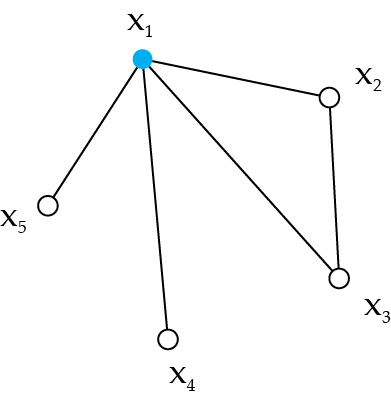
\includegraphics[width=.31\linewidth]{figures/ind-set1.png}} \quad
    \subfloat
    {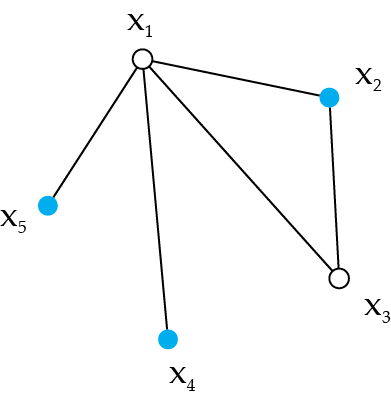
\includegraphics[width=.31\linewidth]{figures/ind-set2.png}} \quad
    \subfloat
    {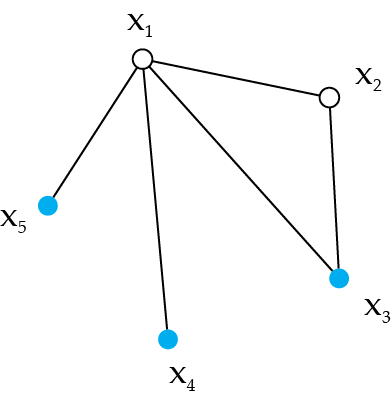
\includegraphics[width=.31\linewidth]{figures/ind-set3.png}} 
    \caption{Three copies of the graph $G$ in \autoref{ex:ind-set}. In each, one of the three maximal independent sets is highlighted in blue.}
\end{figure}
Since we have a simplicial complex, we can construct a Stanley-Reisner ideal that corresponds to the independence complex of $G$. From the way that $\ind (G)$ is constructed, the Stanley-Reisner is actually quite easy to describe. If $\Delta$ is the independence complex of some graph $G$, then its corresponding Stanley-Reisner ideal is that which is generated by monomials of the form $x_i x_j$, where $\br{x_i, x_j}$ is an edge of $G$. In more direct terms, since the faces of $\Delta = \ind (G)$ are exactly those subsets of $V(G)$ which do not share an edge, by definition the non-faces would be those subsets of $V(G)$ that do share an edge. This type of Stanley-Reisner ideal is called the \textbf{edge ideal} of $G$, denoted $I(G)$. That is, the ideal generated by the degree two squarefree monomials that correspond to an edge of $G$:
$$
I(G) := I_\Delta =  \ang{ x_i x_j \, |\, \br{x_i, x_j} \in E(G)}.
$$
Following through with our previous example yields the ideal
$$
I(G) = \ang{x_1 x_2,\,  x_1 x_3, \, x_1 x_4, \, x_1 x_5, \, x_2 x_3}.
$$
\end{example} 
Notice that we have a bijective correspondence between edge ideals in the polynomial ring in $n$ indeterminates $R = k[x_1, \dots, x_n]$ and simple graphs on $n$ vertices. The degree two squarefree monomials that generate the edge ideal uniquely define a graph on $n$ vertices, and vice-versa. 

Using the independence complex of a graph on $n$ vertices as a simplicial complex on the vertex set $\br{x_1, \dots, x_n}$ therefore allows us to construct artinian rings $A(\Delta, a_1, \dots, a_n)$, and there may exist certain choices of $(a_1, \dots, a_n)$ such that the resulting artinian ring is level. For the remainder of this report, we will investigate this special case in which the simplicial complex is the independence complex of a graph. In particular, we will explore the following question:

\begin{question*}
For what graphs $G$ is the independence complex $\Delta = \ind (G)$ levelable?
\end{question*}

Since each graph has a unique independence complex, we can think of levelability as a property of the graph, which gives us the following definition of a levelable graph.

\begin{definition}
A graph $G$ is \textbf{levelable} if its independence complex $\ind(G)$ is levelable. 
\end{definition}


\section{The levelable condition on disconnected graphs} \label{sec:disconnected}

In this section, we will show that the levelability of a graph depends entirely on the levelability of its connected components. That is, a graph is levelable if and only if its connected components are levelable.  This result drastically decreases the number of graphs that we need to check computationally, as well as reduces the problem of proving criteria. We begin by first defining graph connectedness.

\begin{definition}
Let $G$ be a graph on $n$ vertices $V(G) = \br{v_1, \dots, v_n}$. We call $G$ \textbf{connected} if, for every two vertices $v_i$, $v_j \in V(G)$ with $i \neq j$, there exists some sequence of edges $\br{v_i, v_{\alpha_1}}, \br{v_{\alpha_1}, v_{\alpha_2}}, \dots, \br{v_{\alpha_k}, v_j}$ that form a path connecting $v_i$ and $v_j$. A graph is \textbf{disconnected} if it is not connected. The \textbf{connected components} $G_1, \cdots G_m$ of $G$ are the maximal connected subgraphs of $G$. That is, each $G_i$ has vertex set $V(G_i) \subseteq V(G)$ such that every two distinct vertices in $V(G_i)$ are connected by a path, and there are no vertices in $V(G) \setminus V(G_i)$ that are adjacent to any vertex in $V(G_i)$. The edge set $E(G_i) \subset E(G)$ consists of all edges between vertices in $V(G_i)$.
\end{definition}

\begin{lemma} \label{lem:ind-sets-union}
Let $G = G_1 \cup G_2$ with $E(G_1) \cap E(G_2) = \emptyset$ and $V(G_1) \cap V(G_2) = \emptyset$. Let $\Delta_1$ denote $\ind(G_1)$, $\Delta_2$ denote $\ind(G_2)$, and $\Delta$ denote $\ind(G)$. If $S \in \Delta_1$ and $T \in \Delta_2$, then $S \cup T \in \Delta$.  
\end{lemma}

\begin{proof} We wish to show that if $v_i$, $v_j \in S \cup T$, then  $\{v_i, v_j\} \not \in E$. 

\noindent
\underline{Case 1}: $v_i \in S$ and $v_j \in S$.
Since $S \in \Delta_1$, it is an independent set, and so no vertices in $S$ share an edge. So $\{v_i, v_j\} \not \in E.$

\noindent
\underline{Case 2}: $v_i \in T$ and $v_j \in T$. 
Since $T \in \Delta_2$, it is an independent set, and so no vertices in $T$ share an edge. So $\{v_i, v_j\} \not \in E$.

\noindent
\underline{Case 3}: $v_i \in S$ and $v_j \in T$. 
If $v_i \in S$ and $v_j \in T$, then $v_i \in G_1$ and $v_j \in G_2$. Since $G_1$ and $G_2$ are disconnected, it must be that $\{ v_i, v_j \} \not \in E$.

Therefore no pair of vertices in $S \cup T$ share an edge, and $S \cup T \in \ind(G)$. 
\end{proof}

\begin{lemma} \label{lem:section-facets}
Suppose $G = G_1 \cup G_2$ with $E(G_1) \cap E(G_2) = \emptyset$ and $V(G_1) \cap V(G_2) = \emptyset$. Let $\Delta_1 = \ind(G_1)$, $\Delta_2 = \ind (G_2)$, and $\Delta = \ind (G)$. If $F(\Delta)$, $F(\Delta_1)$ and $F(\Delta_2)$ denote the facets of $\Delta$, $\Delta_1$ and $\Delta_2$ respectively, then $$F(\Delta) = \br{ F \cup H \, | \, F \in F(\Delta_1) , \, H \in F(\Delta_2)}.$$
\end{lemma}

\begin{proof}
Let $F \in F(\Delta_1)$ and $H \in F(\Delta_2)$. Then we need to show that any $F \cup H$ is an independent set in $\Delta$ that is maximal under inclusion.

First, notice that any element of $F(\Delta_1)$ or $F(\Delta_2)$ is an independent set in $\Delta$.
Therefore, by \autoref{lem:ind-sets-union} , $F \cup H \in \Delta$.

Now, we show that this is a maximal independent set; that is, if we take any additional vertex $v' \in G$ but $v' \not \in F \cup H$, then $F \cup H \cup \br{v'}$ fails to be an independent set.

Suppose for a contradiction that $F \cup H \cup \br{v'}$ was an independent set. Since $v' \in G$, either $v' \in G_1$ or $v' \in G_2$.  Without loss of generality, suppose $v' \in G_1$. By definition of the independent set, $v'$ does not share an edge with any vertex from $F \cup H$. In particular, it does not share any edges with any vertex in $F$. Then $F \cup \br{v'}$ is an independent set of $G_1$, and thus in $\Delta_1$.

We then have that $F \cup \{v'\} \in \Delta_1$ with $F \subsetneq F \cup \{v'\}$. But this contradicts $F$ being a facet of $\Delta_1$. So $F \cup H$ is a maximal independent set.

To see that these are the only facets of $\Delta$, consider some $F \in F(\Delta)$. We can express $F$ as a union of an independent set $S$ of vertices from $G_1$ and an independent set $T$ of vertices from $G_2$. Since $F$ is maximal, no vertex from $G = G_1 \cup G_2$ can be added to $F$ such that $F$ remains an independent set. 

That is, no vertex from $G_1$ can be added to $S$ so that $S$ is still an independent set, and no vertex from $G_2$ can be added to $T$ so that $T$ is still an independent set. Therefore $S$ and $T$ are maximal under inclusion, and are facets of $\Delta_1$ and $\Delta_2$ respectively.
\end{proof}

\begin{theorem} \label{thm:disconnected-1}
Suppose $G = G_1 \cup G_2$ with $E(G_1) \cap E(G_2) = \emptyset$ and $V(G_1) \cap V(G_2) = \emptyset$. Then $\Delta = \ind(G)$ is levelable if and only if $\Delta_1 = \ind(G_1)$ and $\Delta_2 = \ind(G_2)$ are both levelable.
\end{theorem}


\begin{proof}
We will first assume that both $\Delta_1$ and $\Delta_2$ are levelable, and prove that $\Delta$ must also be levelable.

Suppose component $G_1$ is a graph on $\alpha$ vertices, and $G_2$ is a graph on $\beta$ vertices. Then $G$ is a graph on $\alpha + \beta$ vertices. Let us the label the vertices of $G$ as $\{ x_1 , \dots , x_\alpha, y_{1} , \dots , y_{\beta} \}$, where the first $\alpha$ vertices are from $G_1$ and the latter $\beta$ are from $G_2$. 

If $F(\Delta_1) = \{ F_1, \dots , \, F_M \}$, and $\Delta_1$ is levelable, then there exists some solution $(a_1, \dots , a_\alpha)$, with $\alpha_i \in \mathbb{Z}$, $a_i \geq 2$ to the following system of $M-1$ equations:
\begin{equation}
\label{eq:G1system}
  \begin{aligned}
	S(F_1) - S(F_2) & = |F_1| - |F_2| \\
	S(F_2) - S(F_3) & = |F_2| - |F_3|\\
	&\vdots \\
	S(F_{M-1}) - S(F_M) & = |F_{M-1}| - |F_{M}|.
  \end{aligned}
\end{equation}
If $F(\Delta_2) = \{ H_{1}, \dots , \, H_N \}$, and $\Delta_2$ is levelable, then there exists some solution $(b_1, \dots , b_\beta)$, with $b_i \in \mathbb{Z}$, $b_i \geq 2$ to the following system of $N-1$ equations:
\begin{equation}
\label{eq:G2system}
  \begin{aligned}
	S(H_1) - S(H_2) & = |H_1| - |H_2| \\
	S(H_2) - S(H_3) & = |H_2| - |H_3|\\
	&\vdots \\
    S(H_{N-1}) - S(H_N)& = |H_{N-1}| - |H_N|.
  \end{aligned}
\end{equation}
By \autoref{lem:section-facets}, we have that $F(\Delta) = \{ F_i \cup H_j \, | \,  1 \leq i \leq M , \, 1 \leq j \leq N \}$. Let us label the elements $K_l$ of $F(\Delta)$ as follows:
\begin{equation} \label{all-facets}
\begin{aligned}
	K_1 &= F_1 \cup H_1 \\
    K_2 &= F_1 \cup H_2 \\
    & \; \vdots \\
    K_{N-1} &= F_1 \cup H_{N-1} \\
    K_N &= F_1 \cup H_N \\
    K_{N+1} &= F_2 \cup H_N \\
    & \; \vdots \\ 
    K_{2N-1} &= F_{2} \cup H_{2} \\
	K_{2N} &= F_{2} \cup H_{1} \\
    K_{2N+1} &= F_{3} \cup H_{1} \\
    & \; \vdots \\
    K_{MN-1} &= F_{M} \cup H_{N-1} \\
    K_{MN} &= F_{M} \cup H_{N}. \\
\end{aligned}
\end{equation}
Now, $\Delta$ is levelable if there is some solution $(z_1, \dots , z_{\alpha + \beta})$ of the following system of $MN - 1$ equations:
\begin{equation}
\label{eq:Gsystem}
  \begin{aligned}
	S(K_1) - S(K_2) & = |K_1| - |K_2| \\
	S(K_2) - S(K_3) & = |K_2| - |K_3| \\
	&\vdots \\
	S(K_{MN - 1}) - S(K_{MN}) x & = |K_{MN-1}| - |K_{MN}|.
  \end{aligned}
\end{equation}
We will show that $(a_1, \dots , a_\alpha,  b_1, \dots,b_\beta)$ is a solution to the system of equations \eqref{eq:Gsystem}. Consider the $t^{\textrm{th}}$ equation in the system $S(K_t) - S(K_{t+1}) = |K_t| - |K_{t+1}|$. \\

\noindent
\underline{Case 1:} $t$ is not a multiple of N. Then we can write $K_t$ and $K_{t+1}$ as either
\begin{equation} \label{eq:K1}
\begin{aligned}
K_t = F_i \cup H_j \; \textrm{and} \; K_{t+1} = K_i \cup H_{j+1}
\end{aligned}
\end{equation}
or
\begin{equation} \label{eq:K2}
\begin{aligned}
K_t = F_i \cup H_j \; \textrm{and} \; K_{t+1} = K_i \cup H_{j-1}.
\end{aligned}
\end{equation}
In the case of \eqref{eq:K1}, the $t^{\textrm{th}}$ equation can be written as
$$
S(F_i \cup H_j) - S(F_i \cup H_{j+1}) = | F_{i} \cup H_{j}| - | F_{i} \cup H_{j+1}|.
$$
Since $F_{i}$ is necessarily disjoint from $H_{j}$ and $H_{j+1}$, we can rewrite this as:
\begin{equation*}
\begin{aligned}
S(F_i) + S(H_j) - S(F_i) - S(H_{j+1}) &=  |F_i| + | H_{j}| - |F_i| - |H_{j+1}|,
\end{aligned}
\end{equation*}
which reduces to
\begin{equation*}
\begin{aligned}
S(H_j) - S(H_{j+1}) &=  | H_{j}| - |H_{j+1}|.
\end{aligned}
\end{equation*}
The resulting equation depends only on vertices from $G_2$ (in particular, it is the $j^{\textrm{th}}$ equation in \eqref{eq:G2system}). Thus $(a_1, \dots, a_\alpha, b_1, \dots, b_\beta)$ is a solution to this equation. 

In the case of \eqref{eq:K2}, the $t^{\textrm{th}}$ equation can be written:
\begin{equation*}
\begin{aligned}
S(F_{i} \cup H_{j}) - S(F_{i} \cup H_{j-1}) = | F_{i} \cup H_{j}| - | F_{i} \cup H_{j-1}|.
\end{aligned}
\end{equation*}
Multiplying by $-1$ yields
$$
S(F_{i} \cup H_{j-1}) - S(F_{i} \cup H_{j}) = | F_{i} \cup H_{j-1}| - | F_{i} \cup H_{j}|.
$$
Again, since $F_i$ is disjoint from $H_{j-1}$ and $H_j$, we can write this as 
\begin{equation*}
\begin{aligned}
S(F_i) + S(H_{j-1}) - S(F_i) - S(H_{j}) &=  |F_i| + | H_{j-1}| - |F_i| - |H_{j}|,
\end{aligned}
\end{equation*}
which reduces to
\begin{equation*}
\begin{aligned}
S(H_{j-1}) - S(H_{j}) &= | H_{j-1}| - |H_{j}|.
\end{aligned}
\end{equation*}
This is the $(j-1)^{\textrm{th}}$ equation in \eqref{eq:G2system}, and thus $(a_1, \dots a_\alpha, b_1, \dots , b_\beta)$ is a solution to this equation, since it only depends on the vertices from $G_2$. \\

\noindent
\underline{Case 2}: $t$ is a multiple of $N$. Then 
$$
K_t = F_i \cup H_j \; \textrm{and} \; K_{t+1} = F_{i+1} \cup H_j,
$$
where either $j=1$ or $j=N$. The $t^{\textrm{th}}$ equation can therefore be written
\begin{equation} \label{eq:N}
\begin{aligned}
S(F_{i} \cup H_{j}) - S(F_{ i+1} \cup H_{j}) = | F_{i} \cup H_{j}| - |F_{i+1} \cup H_{j}|,
\end{aligned}
\end{equation}
and since $H_j$ is disjoint from $F_i$ and $F_{i+1}$, we can write this as
\begin{equation*}
\begin{aligned}
S(F_{i}) + S(H_{j}) -  S(F_{i+1})  -S(H_{j})  &= | F_{i} | + | H_{j}| - | F_{i+1}| - |H_{j}|.
\end{aligned}
\end{equation*}
This reduces to
\begin{equation*}
\begin{aligned}
S(F_{i})-   S(F_{i+1})   &= | F_{i} | - | F_{i+1}|,
\end{aligned}
\end{equation*}
which is the $i^{\textrm{th}}$ equation in \eqref{eq:G1system} and concerns only the $\alpha$ vertices from $G_1$, and so we have that $(a_1, \dots, a_\alpha, b_1, \dots,  b_\beta)$ is a solution to the equation.

We then have that $(a_1, \dots, a_\alpha, b_1, \dots, b_\beta)$ is a simultaneous solution to the system of equations \eqref{eq:Gsystem}, and $\Delta$ is levelable. \\


Now, we prove the other direction. That is, if $\Delta_1$ or $\Delta_2$ fail to be levelable, then $\Delta$ is also not levelable. Without loss of generality, assume that $\Delta_1$ is not levelable. Label the facets of $\Delta$ as in \eqref{all-facets}. If we consider every $t^{\textrm{th}}$ equation where $t$ is a multiple of $N$, similar to \eqref{eq:N} we can reduce each equation to the form
\begin{equation}
\begin{aligned}
S(F_i) - S(F_{i+1}) = |F_i| - |F_{i+1}|. 
\end{aligned}
\end{equation}
Applying this to every $N^{\textrm{th}}$ equation in system \eqref{eq:Gsystem} returns the $M-1$ equations in \eqref{eq:G1system} which depends exclusively on vertices in $G_1$. Since $\Delta_1$ is assumed to fail to be levelable, there is no valid choice of $(a_1, \dots, a_\alpha)$ that simultaneously satisfies these $M-1$ equations, and there is therefore no simultaneous solution to the system of $MN-1$ equations. Therefore $G$ is not levelable. 
\end{proof}

\begin{theorem} \label{thm:disconnected-iff}
Let $G$ a graph with connected components $G_1, \dots, G_m$. Then $G$ is levelable if and only if each of its individual connected components are levelable.
\end{theorem}

\begin{proof}
Suppose that $G$ is levelable. For any $i$, $G \setminus G_i$ and $G_i$ satisfy the condition for $G_1$ and $G_2$ in \autoref{thm:disconnected-1}. Therefore $G_i$ must be levelable. Since the choice of $i$ was arbitrary, each of $G_1, \dots, G_m$ is individually levelable.

Now suppose that each of $G_1$ is levelable. Define $H_k = \bigcup_{i = 1}^k G_i$. We will show that $G$ is levelable by an induction argument. The base case is true since $H_1 = G_1$ is levelable by assumption. For the induction step, suppose that $H_{k-1}$ is levelable. Then $H_k = H_{k-1} \cup G_k$ is levelable by \autoref{thm:disconnected-1}, since $G_k$ is levelable.

Therefore $H_k$ is levelable for $i = 1, \dots, m$. In particular, $H_m = G_1 \cup \cdots \cup G_m = G$ is levelable, as required.
\end{proof}

\autoref{thm:disconnected-iff} tells us that the levelability of disconneted graphs depends completely on the levelability on all of its connected components. Therefore, for the rest of this document we will consider only connected graphs, keeping in mind that all these results can easily be extended to all simple graphs.